\documentclass[twoside]{book}

% Packages required by doxygen
\usepackage{fixltx2e}
\usepackage{calc}
\usepackage{doxygen}
\usepackage[export]{adjustbox} % also loads graphicx
\usepackage{graphicx}
\usepackage[utf8]{inputenc}
\usepackage{makeidx}
\usepackage{multicol}
\usepackage{multirow}
\PassOptionsToPackage{warn}{textcomp}
\usepackage{textcomp}
\usepackage[nointegrals]{wasysym}
\usepackage[table]{xcolor}

% Font selection
\usepackage[T1]{fontenc}
\usepackage[scaled=.90]{helvet}
\usepackage{courier}
\usepackage{amssymb}
\usepackage{sectsty}
\renewcommand{\familydefault}{\sfdefault}
\allsectionsfont{%
  \fontseries{bc}\selectfont%
  \color{darkgray}%
}
\renewcommand{\DoxyLabelFont}{%
  \fontseries{bc}\selectfont%
  \color{darkgray}%
}
\newcommand{\+}{\discretionary{\mbox{\scriptsize$\hookleftarrow$}}{}{}}

% Page & text layout
\usepackage{geometry}
\geometry{%
  a4paper,%
  top=2.5cm,%
  bottom=2.5cm,%
  left=2.5cm,%
  right=2.5cm%
}
\tolerance=750
\hfuzz=15pt
\hbadness=750
\setlength{\emergencystretch}{15pt}
\setlength{\parindent}{0cm}
\setlength{\parskip}{3ex plus 2ex minus 2ex}
\makeatletter
\renewcommand{\paragraph}{%
  \@startsection{paragraph}{4}{0ex}{-1.0ex}{1.0ex}{%
    \normalfont\normalsize\bfseries\SS@parafont%
  }%
}
\renewcommand{\subparagraph}{%
  \@startsection{subparagraph}{5}{0ex}{-1.0ex}{1.0ex}{%
    \normalfont\normalsize\bfseries\SS@subparafont%
  }%
}
\makeatother

% Headers & footers
\usepackage{fancyhdr}
\pagestyle{fancyplain}
\fancyhead[LE]{\fancyplain{}{\bfseries\thepage}}
\fancyhead[CE]{\fancyplain{}{}}
\fancyhead[RE]{\fancyplain{}{\bfseries\leftmark}}
\fancyhead[LO]{\fancyplain{}{\bfseries\rightmark}}
\fancyhead[CO]{\fancyplain{}{}}
\fancyhead[RO]{\fancyplain{}{\bfseries\thepage}}
\fancyfoot[LE]{\fancyplain{}{}}
\fancyfoot[CE]{\fancyplain{}{}}
\fancyfoot[RE]{\fancyplain{}{\bfseries\scriptsize Generated by Doxygen }}
\fancyfoot[LO]{\fancyplain{}{\bfseries\scriptsize Generated by Doxygen }}
\fancyfoot[CO]{\fancyplain{}{}}
\fancyfoot[RO]{\fancyplain{}{}}
\renewcommand{\footrulewidth}{0.4pt}
\renewcommand{\chaptermark}[1]{%
  \markboth{#1}{}%
}
\renewcommand{\sectionmark}[1]{%
  \markright{\thesection\ #1}%
}

% Indices & bibliography
\usepackage{natbib}
\usepackage[titles]{tocloft}
\setcounter{tocdepth}{3}
\setcounter{secnumdepth}{5}
\makeindex

% Hyperlinks (required, but should be loaded last)
\usepackage{ifpdf}
\ifpdf
  \usepackage[pdftex,pagebackref=true]{hyperref}
\else
  \usepackage[ps2pdf,pagebackref=true]{hyperref}
\fi
\hypersetup{%
  colorlinks=true,%
  linkcolor=blue,%
  citecolor=blue,%
  unicode%
}

% Custom commands
\newcommand{\clearemptydoublepage}{%
  \newpage{\pagestyle{empty}\cleardoublepage}%
}

\usepackage{caption}
\captionsetup{labelsep=space,justification=centering,font={bf},singlelinecheck=off,skip=4pt,position=top}

%===== C O N T E N T S =====

\begin{document}

% Titlepage & ToC
\hypersetup{pageanchor=false,
             bookmarksnumbered=true,
             pdfencoding=unicode
            }
\pagenumbering{roman}
\begin{titlepage}
\vspace*{7cm}
\begin{center}%
{\Large Heisprosjekt gruppe 5 }\\
\vspace*{1cm}
{\large Generated by Doxygen 1.8.11}\\
\end{center}
\end{titlepage}
\clearemptydoublepage
\tableofcontents
\clearemptydoublepage
\pagenumbering{arabic}
\hypersetup{pageanchor=true}

%--- Begin generated contents ---
\chapter{File Index}
\section{File List}
Here is a list of all documented files with brief descriptions\+:\begin{DoxyCompactList}
\item\contentsline{section}{source/{\bfseries .\+c} }{\pageref{_8c}}{}
\item\contentsline{section}{source/{\bfseries channels.\+h} }{\pageref{channels_8h}}{}
\item\contentsline{section}{source/{\bfseries elev.\+c} }{\pageref{elev_8c}}{}
\item\contentsline{section}{source/\hyperlink{elev_8h}{elev.\+h} \\*A simple library for doing operations on memory buffers consisting of integers }{\pageref{elev_8h}}{}
\item\contentsline{section}{source/{\bfseries io.\+c} }{\pageref{io_8c}}{}
\item\contentsline{section}{source/{\bfseries io.\+h} }{\pageref{io_8h}}{}
\item\contentsline{section}{source/{\bfseries main.\+c} }{\pageref{main_8c}}{}
\item\contentsline{section}{source/{\bfseries orders.\+c} }{\pageref{orders_8c}}{}
\item\contentsline{section}{source/\hyperlink{orders_8h}{orders.\+h} \\*A simple library for doing operations on memory buffers consisting of integers }{\pageref{orders_8h}}{}
\item\contentsline{section}{source/{\bfseries queue.\+c} }{\pageref{queue_8c}}{}
\item\contentsline{section}{source/\hyperlink{queue_8h}{queue.\+h} \\*A simple library for doing operations on memory buffers consisting of integers }{\pageref{queue_8h}}{}
\item\contentsline{section}{source/{\bfseries timer.\+c} }{\pageref{timer_8c}}{}
\item\contentsline{section}{source/\hyperlink{timer_8h}{timer.\+h} \\*A simple library for doing operations on memory buffers consisting of integers }{\pageref{timer_8h}}{}
\end{DoxyCompactList}

\chapter{File Documentation}
\hypertarget{elev_8h}{}\section{source/elev.h File Reference}
\label{elev_8h}\index{source/elev.\+h@{source/elev.\+h}}


A simple library for doing operations on memory buffers consisting of integers.  


This graph shows which files directly or indirectly include this file\+:\nopagebreak
\begin{figure}[H]
\begin{center}
\leavevmode
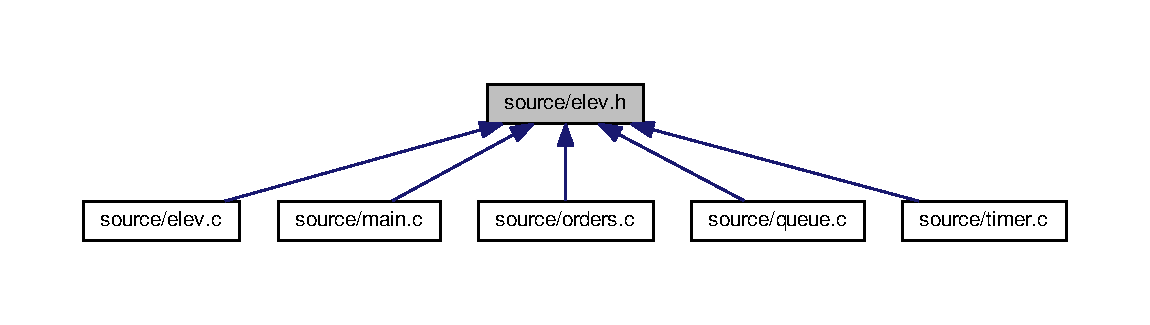
\includegraphics[width=350pt]{elev_8h__dep__incl}
\end{center}
\end{figure}
\subsection*{Macros}
\begin{DoxyCompactItemize}
\item 
\#define {\bfseries N\+\_\+\+F\+L\+O\+O\+RS}~4\hypertarget{elev_8h_ae0592e3739e5e1e76234bb1caf9d1305}{}\label{elev_8h_ae0592e3739e5e1e76234bb1caf9d1305}

\item 
\#define {\bfseries N\+\_\+\+B\+U\+T\+T\+O\+NS}~3\hypertarget{elev_8h_a271dda243b0f5bd7d2053d258eb71962}{}\label{elev_8h_a271dda243b0f5bd7d2053d258eb71962}

\end{DoxyCompactItemize}
\subsection*{Typedefs}
\begin{DoxyCompactItemize}
\item 
typedef enum \hyperlink{elev_8h_aaf85d173ea1bbd3d99c5a2fcf58cba11}{tag\+\_\+elev\+\_\+motor\+\_\+direction} \hyperlink{elev_8h_a2256dfd58fecce253106f83fd2ed607f}{elev\+\_\+motor\+\_\+direction\+\_\+t}
\item 
typedef enum \hyperlink{elev_8h_a0c3f8374e6ebcc71f91341eb3ba6f6f9}{tag\+\_\+elev\+\_\+lamp\+\_\+type} \hyperlink{elev_8h_af61c4136fb437a2c49037e5a57c9abda}{elev\+\_\+button\+\_\+type\+\_\+t}
\end{DoxyCompactItemize}
\subsection*{Enumerations}
\begin{DoxyCompactItemize}
\item 
enum \hyperlink{elev_8h_aaf85d173ea1bbd3d99c5a2fcf58cba11}{tag\+\_\+elev\+\_\+motor\+\_\+direction} \{ {\bfseries D\+I\+R\+N\+\_\+\+D\+O\+WN} = -\/1, 
{\bfseries D\+I\+R\+N\+\_\+\+S\+T\+OP} = 0, 
{\bfseries D\+I\+R\+N\+\_\+\+UP} = 1
 \}
\item 
enum \hyperlink{elev_8h_a0c3f8374e6ebcc71f91341eb3ba6f6f9}{tag\+\_\+elev\+\_\+lamp\+\_\+type} \{ {\bfseries B\+U\+T\+T\+O\+N\+\_\+\+C\+A\+L\+L\+\_\+\+UP} = 0, 
{\bfseries B\+U\+T\+T\+O\+N\+\_\+\+C\+A\+L\+L\+\_\+\+D\+O\+WN} = 1, 
{\bfseries B\+U\+T\+T\+O\+N\+\_\+\+C\+O\+M\+M\+A\+ND} = 2
 \}
\end{DoxyCompactItemize}
\subsection*{Functions}
\begin{DoxyCompactItemize}
\item 
int \hyperlink{elev_8h_a949b0e1f7c0f03ea6f92008c378e4573}{elev\+\_\+init} (void)
\item 
void \hyperlink{elev_8h_ac7dccb879f6e812e9d245174a0214536}{elev\+\_\+set\+\_\+motor\+\_\+direction} (\hyperlink{elev_8h_a2256dfd58fecce253106f83fd2ed607f}{elev\+\_\+motor\+\_\+direction\+\_\+t} dirn)
\item 
void \hyperlink{elev_8h_a6ce9a34b8677b483b0d8f9dc47b42c40}{elev\+\_\+set\+\_\+door\+\_\+open\+\_\+lamp} (int value)
\item 
int \hyperlink{elev_8h_acd97a0fbc9013dc954923e25e90be9df}{elev\+\_\+get\+\_\+obstruction\+\_\+signal} (void)
\item 
int \hyperlink{elev_8h_ab702d0ff2d7d03172b7ae3829ba13028}{elev\+\_\+get\+\_\+stop\+\_\+signal} (void)
\item 
void \hyperlink{elev_8h_a85de2a6536b4dd0c83bac19923500740}{elev\+\_\+set\+\_\+stop\+\_\+lamp} (int value)
\item 
int \hyperlink{elev_8h_a97d30b7e2538acf5647515638070fdc5}{elev\+\_\+get\+\_\+floor\+\_\+sensor\+\_\+signal} (void)
\item 
void \hyperlink{elev_8h_a6af53dd3ebae3a5791ba345eac84d4be}{elev\+\_\+set\+\_\+floor\+\_\+indicator} (int floor)
\item 
int \hyperlink{elev_8h_a2350a1635233760719700552a6cb0763}{elev\+\_\+get\+\_\+button\+\_\+signal} (\hyperlink{elev_8h_af61c4136fb437a2c49037e5a57c9abda}{elev\+\_\+button\+\_\+type\+\_\+t} button, int floor)
\item 
void \hyperlink{elev_8h_a9e81321c63d80ddf1699bc91593cd9d4}{elev\+\_\+set\+\_\+button\+\_\+lamp} (\hyperlink{elev_8h_af61c4136fb437a2c49037e5a57c9abda}{elev\+\_\+button\+\_\+type\+\_\+t} button, int floor, int value)
\item 
int \hyperlink{elev_8h_af5d1e754314b8303f2e134187da9b92b}{elev\+\_\+check\+\_\+order} ()
\item 
int \hyperlink{elev_8h_a42577299dbc16c5528694d5f061e5b1b}{elev\+\_\+get\+\_\+floor} ()
\item 
int \hyperlink{elev_8h_ab95114e5ad44dda6d447ff333b1ef0bc}{elev\+\_\+get\+\_\+button\+\_\+type} ()
\end{DoxyCompactItemize}


\subsection{Detailed Description}
A simple library for doing operations on memory buffers consisting of integers. 



\subsection{Typedef Documentation}
\index{elev.\+h@{elev.\+h}!elev\+\_\+button\+\_\+type\+\_\+t@{elev\+\_\+button\+\_\+type\+\_\+t}}
\index{elev\+\_\+button\+\_\+type\+\_\+t@{elev\+\_\+button\+\_\+type\+\_\+t}!elev.\+h@{elev.\+h}}
\subsubsection[{\texorpdfstring{elev\+\_\+button\+\_\+type\+\_\+t}{elev_button_type_t}}]{\setlength{\rightskip}{0pt plus 5cm}typedef enum {\bf tag\+\_\+elev\+\_\+lamp\+\_\+type}  {\bf elev\+\_\+button\+\_\+type\+\_\+t}}\hypertarget{elev_8h_af61c4136fb437a2c49037e5a57c9abda}{}\label{elev_8h_af61c4136fb437a2c49037e5a57c9abda}
Button types for function \hyperlink{elev_8h_a9e81321c63d80ddf1699bc91593cd9d4}{elev\+\_\+set\+\_\+button\+\_\+lamp()} and elev\+\_\+get\+\_\+button(). \index{elev.\+h@{elev.\+h}!elev\+\_\+motor\+\_\+direction\+\_\+t@{elev\+\_\+motor\+\_\+direction\+\_\+t}}
\index{elev\+\_\+motor\+\_\+direction\+\_\+t@{elev\+\_\+motor\+\_\+direction\+\_\+t}!elev.\+h@{elev.\+h}}
\subsubsection[{\texorpdfstring{elev\+\_\+motor\+\_\+direction\+\_\+t}{elev_motor_direction_t}}]{\setlength{\rightskip}{0pt plus 5cm}typedef enum {\bf tag\+\_\+elev\+\_\+motor\+\_\+direction}  {\bf elev\+\_\+motor\+\_\+direction\+\_\+t}}\hypertarget{elev_8h_a2256dfd58fecce253106f83fd2ed607f}{}\label{elev_8h_a2256dfd58fecce253106f83fd2ed607f}
Motor direction for function \hyperlink{elev_8h_ac7dccb879f6e812e9d245174a0214536}{elev\+\_\+set\+\_\+motor\+\_\+direction()}. 

\subsection{Enumeration Type Documentation}
\index{elev.\+h@{elev.\+h}!tag\+\_\+elev\+\_\+lamp\+\_\+type@{tag\+\_\+elev\+\_\+lamp\+\_\+type}}
\index{tag\+\_\+elev\+\_\+lamp\+\_\+type@{tag\+\_\+elev\+\_\+lamp\+\_\+type}!elev.\+h@{elev.\+h}}
\subsubsection[{\texorpdfstring{tag\+\_\+elev\+\_\+lamp\+\_\+type}{tag_elev_lamp_type}}]{\setlength{\rightskip}{0pt plus 5cm}enum {\bf tag\+\_\+elev\+\_\+lamp\+\_\+type}}\hypertarget{elev_8h_a0c3f8374e6ebcc71f91341eb3ba6f6f9}{}\label{elev_8h_a0c3f8374e6ebcc71f91341eb3ba6f6f9}
Button types for function \hyperlink{elev_8h_a9e81321c63d80ddf1699bc91593cd9d4}{elev\+\_\+set\+\_\+button\+\_\+lamp()} and elev\+\_\+get\+\_\+button(). 

Definition at line 105 of file elev.\+h.

\index{elev.\+h@{elev.\+h}!tag\+\_\+elev\+\_\+motor\+\_\+direction@{tag\+\_\+elev\+\_\+motor\+\_\+direction}}
\index{tag\+\_\+elev\+\_\+motor\+\_\+direction@{tag\+\_\+elev\+\_\+motor\+\_\+direction}!elev.\+h@{elev.\+h}}
\subsubsection[{\texorpdfstring{tag\+\_\+elev\+\_\+motor\+\_\+direction}{tag_elev_motor_direction}}]{\setlength{\rightskip}{0pt plus 5cm}enum {\bf tag\+\_\+elev\+\_\+motor\+\_\+direction}}\hypertarget{elev_8h_aaf85d173ea1bbd3d99c5a2fcf58cba11}{}\label{elev_8h_aaf85d173ea1bbd3d99c5a2fcf58cba11}
Motor direction for function \hyperlink{elev_8h_ac7dccb879f6e812e9d245174a0214536}{elev\+\_\+set\+\_\+motor\+\_\+direction()}. 

Definition at line 37 of file elev.\+h.



\subsection{Function Documentation}
\index{elev.\+h@{elev.\+h}!elev\+\_\+check\+\_\+order@{elev\+\_\+check\+\_\+order}}
\index{elev\+\_\+check\+\_\+order@{elev\+\_\+check\+\_\+order}!elev.\+h@{elev.\+h}}
\subsubsection[{\texorpdfstring{elev\+\_\+check\+\_\+order()}{elev_check_order()}}]{\setlength{\rightskip}{0pt plus 5cm}int elev\+\_\+check\+\_\+order (
\begin{DoxyParamCaption}
{}
\end{DoxyParamCaption}
)}\hypertarget{elev_8h_af5d1e754314b8303f2e134187da9b92b}{}\label{elev_8h_af5d1e754314b8303f2e134187da9b92b}
Checks if a button is pressed. \begin{DoxyReturn}{Returns}
1 if button is pressed, 0 if not. 
\end{DoxyReturn}


Definition at line 158 of file elev.\+c.

\index{elev.\+h@{elev.\+h}!elev\+\_\+get\+\_\+button\+\_\+signal@{elev\+\_\+get\+\_\+button\+\_\+signal}}
\index{elev\+\_\+get\+\_\+button\+\_\+signal@{elev\+\_\+get\+\_\+button\+\_\+signal}!elev.\+h@{elev.\+h}}
\subsubsection[{\texorpdfstring{elev\+\_\+get\+\_\+button\+\_\+signal(elev\+\_\+button\+\_\+type\+\_\+t button, int floor)}{elev_get_button_signal(elev_button_type_t button, int floor)}}]{\setlength{\rightskip}{0pt plus 5cm}int elev\+\_\+get\+\_\+button\+\_\+signal (
\begin{DoxyParamCaption}
\item[{{\bf elev\+\_\+button\+\_\+type\+\_\+t}}]{button, }
\item[{int}]{floor}
\end{DoxyParamCaption}
)}\hypertarget{elev_8h_a2350a1635233760719700552a6cb0763}{}\label{elev_8h_a2350a1635233760719700552a6cb0763}
Gets a button signal. 
\begin{DoxyParams}{Parameters}
{\em button} & Which button type to check. Can be B\+U\+T\+T\+O\+N\+\_\+\+C\+A\+L\+L\+\_\+\+UP, B\+U\+T\+T\+O\+N\+\_\+\+C\+A\+L\+L\+\_\+\+D\+O\+WN or B\+U\+T\+T\+O\+N\+\_\+\+C\+O\+M\+M\+A\+ND (button "inside the elevator). \\
\hline
{\em floor} & Which floor to check button. Must be 0-\/3. \\
\hline
\end{DoxyParams}
\begin{DoxyReturn}{Returns}
0 if button is not pushed. 1 if button is pushed. 
\end{DoxyReturn}


Definition at line 132 of file elev.\+c.

\index{elev.\+h@{elev.\+h}!elev\+\_\+get\+\_\+button\+\_\+type@{elev\+\_\+get\+\_\+button\+\_\+type}}
\index{elev\+\_\+get\+\_\+button\+\_\+type@{elev\+\_\+get\+\_\+button\+\_\+type}!elev.\+h@{elev.\+h}}
\subsubsection[{\texorpdfstring{elev\+\_\+get\+\_\+button\+\_\+type()}{elev_get_button_type()}}]{\setlength{\rightskip}{0pt plus 5cm}int elev\+\_\+get\+\_\+button\+\_\+type (
\begin{DoxyParamCaption}
{}
\end{DoxyParamCaption}
)}\hypertarget{elev_8h_ab95114e5ad44dda6d447ff333b1ef0bc}{}\label{elev_8h_ab95114e5ad44dda6d447ff333b1ef0bc}
Gets the type of button pressed in an order \begin{DoxyReturn}{Returns}
Returns the button type in order 
\end{DoxyReturn}


Definition at line 179 of file elev.\+c.

\index{elev.\+h@{elev.\+h}!elev\+\_\+get\+\_\+floor@{elev\+\_\+get\+\_\+floor}}
\index{elev\+\_\+get\+\_\+floor@{elev\+\_\+get\+\_\+floor}!elev.\+h@{elev.\+h}}
\subsubsection[{\texorpdfstring{elev\+\_\+get\+\_\+floor()}{elev_get_floor()}}]{\setlength{\rightskip}{0pt plus 5cm}int elev\+\_\+get\+\_\+floor (
\begin{DoxyParamCaption}
{}
\end{DoxyParamCaption}
)}\hypertarget{elev_8h_a42577299dbc16c5528694d5f061e5b1b}{}\label{elev_8h_a42577299dbc16c5528694d5f061e5b1b}
Gets the floor where thre is an order \begin{DoxyReturn}{Returns}
Returns the floor where there is an order 
\end{DoxyReturn}


Definition at line 175 of file elev.\+c.

\index{elev.\+h@{elev.\+h}!elev\+\_\+get\+\_\+floor\+\_\+sensor\+\_\+signal@{elev\+\_\+get\+\_\+floor\+\_\+sensor\+\_\+signal}}
\index{elev\+\_\+get\+\_\+floor\+\_\+sensor\+\_\+signal@{elev\+\_\+get\+\_\+floor\+\_\+sensor\+\_\+signal}!elev.\+h@{elev.\+h}}
\subsubsection[{\texorpdfstring{elev\+\_\+get\+\_\+floor\+\_\+sensor\+\_\+signal(void)}{elev_get_floor_sensor_signal(void)}}]{\setlength{\rightskip}{0pt plus 5cm}int elev\+\_\+get\+\_\+floor\+\_\+sensor\+\_\+signal (
\begin{DoxyParamCaption}
\item[{void}]{}
\end{DoxyParamCaption}
)}\hypertarget{elev_8h_a97d30b7e2538acf5647515638070fdc5}{}\label{elev_8h_a97d30b7e2538acf5647515638070fdc5}
Get floor sensor signal. \begin{DoxyReturn}{Returns}
-\/1 if elevator is not on a floor. 0-\/3 if elevator is on floor. 0 is ground floor, 3 is top floor. 
\end{DoxyReturn}


Definition at line 103 of file elev.\+c.

\index{elev.\+h@{elev.\+h}!elev\+\_\+get\+\_\+obstruction\+\_\+signal@{elev\+\_\+get\+\_\+obstruction\+\_\+signal}}
\index{elev\+\_\+get\+\_\+obstruction\+\_\+signal@{elev\+\_\+get\+\_\+obstruction\+\_\+signal}!elev.\+h@{elev.\+h}}
\subsubsection[{\texorpdfstring{elev\+\_\+get\+\_\+obstruction\+\_\+signal(void)}{elev_get_obstruction_signal(void)}}]{\setlength{\rightskip}{0pt plus 5cm}int elev\+\_\+get\+\_\+obstruction\+\_\+signal (
\begin{DoxyParamCaption}
\item[{void}]{}
\end{DoxyParamCaption}
)}\hypertarget{elev_8h_acd97a0fbc9013dc954923e25e90be9df}{}\label{elev_8h_acd97a0fbc9013dc954923e25e90be9df}
Get signal from obstruction switch. \begin{DoxyReturn}{Returns}
1 if obstruction is enabled. 0 if not. 
\end{DoxyReturn}


Definition at line 88 of file elev.\+c.

\index{elev.\+h@{elev.\+h}!elev\+\_\+get\+\_\+stop\+\_\+signal@{elev\+\_\+get\+\_\+stop\+\_\+signal}}
\index{elev\+\_\+get\+\_\+stop\+\_\+signal@{elev\+\_\+get\+\_\+stop\+\_\+signal}!elev.\+h@{elev.\+h}}
\subsubsection[{\texorpdfstring{elev\+\_\+get\+\_\+stop\+\_\+signal(void)}{elev_get_stop_signal(void)}}]{\setlength{\rightskip}{0pt plus 5cm}int elev\+\_\+get\+\_\+stop\+\_\+signal (
\begin{DoxyParamCaption}
\item[{void}]{}
\end{DoxyParamCaption}
)}\hypertarget{elev_8h_ab702d0ff2d7d03172b7ae3829ba13028}{}\label{elev_8h_ab702d0ff2d7d03172b7ae3829ba13028}
Get signal from stop button. \begin{DoxyReturn}{Returns}
1 if stop button is pushed, 0 if not. 
\end{DoxyReturn}


Definition at line 92 of file elev.\+c.

\index{elev.\+h@{elev.\+h}!elev\+\_\+init@{elev\+\_\+init}}
\index{elev\+\_\+init@{elev\+\_\+init}!elev.\+h@{elev.\+h}}
\subsubsection[{\texorpdfstring{elev\+\_\+init(void)}{elev_init(void)}}]{\setlength{\rightskip}{0pt plus 5cm}int elev\+\_\+init (
\begin{DoxyParamCaption}
\item[{void}]{}
\end{DoxyParamCaption}
)}\hypertarget{elev_8h_a949b0e1f7c0f03ea6f92008c378e4573}{}\label{elev_8h_a949b0e1f7c0f03ea6f92008c378e4573}
Initialize elevator. \begin{DoxyReturn}{Returns}
Non-\/zero on success, 0 on failure. 
\end{DoxyReturn}


Definition at line 35 of file elev.\+c.

\index{elev.\+h@{elev.\+h}!elev\+\_\+set\+\_\+button\+\_\+lamp@{elev\+\_\+set\+\_\+button\+\_\+lamp}}
\index{elev\+\_\+set\+\_\+button\+\_\+lamp@{elev\+\_\+set\+\_\+button\+\_\+lamp}!elev.\+h@{elev.\+h}}
\subsubsection[{\texorpdfstring{elev\+\_\+set\+\_\+button\+\_\+lamp(elev\+\_\+button\+\_\+type\+\_\+t button, int floor, int value)}{elev_set_button_lamp(elev_button_type_t button, int floor, int value)}}]{\setlength{\rightskip}{0pt plus 5cm}void elev\+\_\+set\+\_\+button\+\_\+lamp (
\begin{DoxyParamCaption}
\item[{{\bf elev\+\_\+button\+\_\+type\+\_\+t}}]{button, }
\item[{int}]{floor, }
\item[{int}]{value}
\end{DoxyParamCaption}
)}\hypertarget{elev_8h_a9e81321c63d80ddf1699bc91593cd9d4}{}\label{elev_8h_a9e81321c63d80ddf1699bc91593cd9d4}
Set a button lamp. 
\begin{DoxyParams}{Parameters}
{\em lamp} & Which type of lamp to set. Can be B\+U\+T\+T\+O\+N\+\_\+\+C\+A\+L\+L\+\_\+\+UP, B\+U\+T\+T\+O\+N\+\_\+\+C\+A\+L\+L\+\_\+\+D\+O\+WN or B\+U\+T\+T\+O\+N\+\_\+\+C\+O\+M\+M\+A\+ND (button \char`\"{}inside\char`\"{} the elevator). \\
\hline
{\em floor} & Floor of lamp to set. Must be 0-\/3 \\
\hline
{\em value} & Non-\/zero value turns lamp on, 0 turns lamp off. \\
\hline
\end{DoxyParams}


Definition at line 145 of file elev.\+c.

\index{elev.\+h@{elev.\+h}!elev\+\_\+set\+\_\+door\+\_\+open\+\_\+lamp@{elev\+\_\+set\+\_\+door\+\_\+open\+\_\+lamp}}
\index{elev\+\_\+set\+\_\+door\+\_\+open\+\_\+lamp@{elev\+\_\+set\+\_\+door\+\_\+open\+\_\+lamp}!elev.\+h@{elev.\+h}}
\subsubsection[{\texorpdfstring{elev\+\_\+set\+\_\+door\+\_\+open\+\_\+lamp(int value)}{elev_set_door_open_lamp(int value)}}]{\setlength{\rightskip}{0pt plus 5cm}void elev\+\_\+set\+\_\+door\+\_\+open\+\_\+lamp (
\begin{DoxyParamCaption}
\item[{int}]{value}
\end{DoxyParamCaption}
)}\hypertarget{elev_8h_a6ce9a34b8677b483b0d8f9dc47b42c40}{}\label{elev_8h_a6ce9a34b8677b483b0d8f9dc47b42c40}
Turn door-\/open lamp on or off. 
\begin{DoxyParams}{Parameters}
{\em value} & Non-\/zero value turns lamp on, 0 turns lamp off. \\
\hline
\end{DoxyParams}


Definition at line 81 of file elev.\+c.

\index{elev.\+h@{elev.\+h}!elev\+\_\+set\+\_\+floor\+\_\+indicator@{elev\+\_\+set\+\_\+floor\+\_\+indicator}}
\index{elev\+\_\+set\+\_\+floor\+\_\+indicator@{elev\+\_\+set\+\_\+floor\+\_\+indicator}!elev.\+h@{elev.\+h}}
\subsubsection[{\texorpdfstring{elev\+\_\+set\+\_\+floor\+\_\+indicator(int floor)}{elev_set_floor_indicator(int floor)}}]{\setlength{\rightskip}{0pt plus 5cm}void elev\+\_\+set\+\_\+floor\+\_\+indicator (
\begin{DoxyParamCaption}
\item[{int}]{floor}
\end{DoxyParamCaption}
)}\hypertarget{elev_8h_a6af53dd3ebae3a5791ba345eac84d4be}{}\label{elev_8h_a6af53dd3ebae3a5791ba345eac84d4be}
Set floor indicator lamp for a given floor. 
\begin{DoxyParams}{Parameters}
{\em floor} & Which floor lamp to turn on. Other floor lamps are turned off. \\
\hline
\end{DoxyParams}


Definition at line 116 of file elev.\+c.

\index{elev.\+h@{elev.\+h}!elev\+\_\+set\+\_\+motor\+\_\+direction@{elev\+\_\+set\+\_\+motor\+\_\+direction}}
\index{elev\+\_\+set\+\_\+motor\+\_\+direction@{elev\+\_\+set\+\_\+motor\+\_\+direction}!elev.\+h@{elev.\+h}}
\subsubsection[{\texorpdfstring{elev\+\_\+set\+\_\+motor\+\_\+direction(elev\+\_\+motor\+\_\+direction\+\_\+t dirn)}{elev_set_motor_direction(elev_motor_direction_t dirn)}}]{\setlength{\rightskip}{0pt plus 5cm}void elev\+\_\+set\+\_\+motor\+\_\+direction (
\begin{DoxyParamCaption}
\item[{{\bf elev\+\_\+motor\+\_\+direction\+\_\+t}}]{dirn}
\end{DoxyParamCaption}
)}\hypertarget{elev_8h_ac7dccb879f6e812e9d245174a0214536}{}\label{elev_8h_ac7dccb879f6e812e9d245174a0214536}
Sets the motor direction of the elevator. 
\begin{DoxyParams}{Parameters}
{\em dirn} & New direction of the elevator. \\
\hline
\end{DoxyParams}


Definition at line 69 of file elev.\+c.

\index{elev.\+h@{elev.\+h}!elev\+\_\+set\+\_\+stop\+\_\+lamp@{elev\+\_\+set\+\_\+stop\+\_\+lamp}}
\index{elev\+\_\+set\+\_\+stop\+\_\+lamp@{elev\+\_\+set\+\_\+stop\+\_\+lamp}!elev.\+h@{elev.\+h}}
\subsubsection[{\texorpdfstring{elev\+\_\+set\+\_\+stop\+\_\+lamp(int value)}{elev_set_stop_lamp(int value)}}]{\setlength{\rightskip}{0pt plus 5cm}void elev\+\_\+set\+\_\+stop\+\_\+lamp (
\begin{DoxyParamCaption}
\item[{int}]{value}
\end{DoxyParamCaption}
)}\hypertarget{elev_8h_a85de2a6536b4dd0c83bac19923500740}{}\label{elev_8h_a85de2a6536b4dd0c83bac19923500740}
Turn stop lamp on or off. 
\begin{DoxyParams}{Parameters}
{\em value} & Non-\/zero value turns lamp on, 0 turns lamp off. \\
\hline
\end{DoxyParams}


Definition at line 96 of file elev.\+c.


\hypertarget{orders_8h}{}\section{source/orders.h File Reference}
\label{orders_8h}\index{source/orders.\+h@{source/orders.\+h}}


Library of functions for linking orders and elevator functionality.  


This graph shows which files directly or indirectly include this file\+:\nopagebreak
\begin{figure}[H]
\begin{center}
\leavevmode
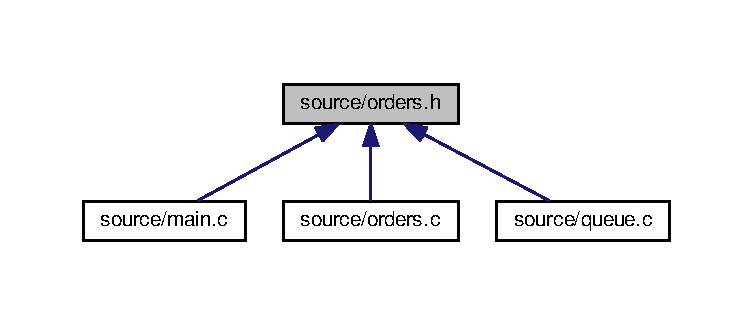
\includegraphics[width=350pt]{orders_8h__dep__incl}
\end{center}
\end{figure}
\subsection*{Functions}
\begin{DoxyCompactItemize}
\item 
void \hyperlink{orders_8h_adddb42a1c068e13a8035daecf4656230}{orders\+\_\+set\+\_\+floor\+\_\+light} ()\hypertarget{orders_8h_adddb42a1c068e13a8035daecf4656230}{}\label{orders_8h_adddb42a1c068e13a8035daecf4656230}

\begin{DoxyCompactList}\small\item\em Sets the floor light for the last visited floor. \end{DoxyCompactList}\item 
void \hyperlink{orders_8h_a08d4a7790768e59d5b6108a67ff3a3e8}{orders\+\_\+start\+\_\+elev} (int direction)
\begin{DoxyCompactList}\small\item\em Starts the elevator in the direction defined by the input parameter. \end{DoxyCompactList}\item 
void \hyperlink{orders_8h_ab46c6a5bc3d1c03fdcad668444daf2e1}{orders\+\_\+open\+\_\+door\+\_\+timed} (int last\+\_\+floor)
\begin{DoxyCompactList}\small\item\em Opens the door for three seconds while recieving orders. \end{DoxyCompactList}\item 
int \hyperlink{orders_8h_ae1a9f09e3aa859db01db65d4b683ebbd}{orders\+\_\+update\+\_\+last\+\_\+floor} (int last\+\_\+floor)
\begin{DoxyCompactList}\small\item\em Update last\+\_\+floor depending on which floor the elevator was in last. \end{DoxyCompactList}\item 
int \hyperlink{orders_8h_a6d2dc16203975cb12c63802b03a4c8bb}{orders\+\_\+set\+\_\+direction} (int direction, int last\+\_\+floor, int next\+\_\+floor)
\begin{DoxyCompactList}\small\item\em Finds the direction which the elevator should be moving next. \end{DoxyCompactList}\item 
int \hyperlink{orders_8h_a6a7c7081c3a77e72473f8c7af2893564}{orders\+\_\+get\+\_\+next\+\_\+floor} (int last\+\_\+floor, int direction)
\begin{DoxyCompactList}\small\item\em Finds the direction which the elevator should be moving next. \end{DoxyCompactList}\item 
void \hyperlink{orders_8h_a741c4d3eb892708577654cb9b93f6fb2}{orders\+\_\+set\+\_\+door\+\_\+lamp} (int value)
\begin{DoxyCompactList}\small\item\em Sets door lamp according to input value. \end{DoxyCompactList}\end{DoxyCompactItemize}


\subsection{Detailed Description}
Library of functions for linking orders and elevator functionality. 



\subsection{Function Documentation}
\index{orders.\+h@{orders.\+h}!orders\+\_\+get\+\_\+next\+\_\+floor@{orders\+\_\+get\+\_\+next\+\_\+floor}}
\index{orders\+\_\+get\+\_\+next\+\_\+floor@{orders\+\_\+get\+\_\+next\+\_\+floor}!orders.\+h@{orders.\+h}}
\subsubsection[{\texorpdfstring{orders\+\_\+get\+\_\+next\+\_\+floor(int last\+\_\+floor, int direction)}{orders_get_next_floor(int last_floor, int direction)}}]{\setlength{\rightskip}{0pt plus 5cm}int orders\+\_\+get\+\_\+next\+\_\+floor (
\begin{DoxyParamCaption}
\item[{int}]{last\+\_\+floor, }
\item[{int}]{direction}
\end{DoxyParamCaption}
)}\hypertarget{orders_8h_a6a7c7081c3a77e72473f8c7af2893564}{}\label{orders_8h_a6a7c7081c3a77e72473f8c7af2893564}


Finds the direction which the elevator should be moving next. 


\begin{DoxyParams}{Parameters}
{\em last\+\_\+floor} & Last floor elevator visited. \\
\hline
{\em direction} & Direction the elevator is headed \\
\hline
\end{DoxyParams}
\begin{DoxyReturn}{Returns}
the next floor the elevator is headed to. 
\end{DoxyReturn}


Definition at line 132 of file orders.\+c.

\index{orders.\+h@{orders.\+h}!orders\+\_\+open\+\_\+door\+\_\+timed@{orders\+\_\+open\+\_\+door\+\_\+timed}}
\index{orders\+\_\+open\+\_\+door\+\_\+timed@{orders\+\_\+open\+\_\+door\+\_\+timed}!orders.\+h@{orders.\+h}}
\subsubsection[{\texorpdfstring{orders\+\_\+open\+\_\+door\+\_\+timed(int last\+\_\+floor)}{orders_open_door_timed(int last_floor)}}]{\setlength{\rightskip}{0pt plus 5cm}void orders\+\_\+open\+\_\+door\+\_\+timed (
\begin{DoxyParamCaption}
\item[{int}]{last\+\_\+floor}
\end{DoxyParamCaption}
)}\hypertarget{orders_8h_ab46c6a5bc3d1c03fdcad668444daf2e1}{}\label{orders_8h_ab46c6a5bc3d1c03fdcad668444daf2e1}


Opens the door for three seconds while recieving orders. 


\begin{DoxyParams}{Parameters}
{\em last\+\_\+floor} & last floor elevator visited in case the elevator ain\textquotesingle{}t at a new one \\
\hline
\end{DoxyParams}


Definition at line 17 of file orders.\+c.

\index{orders.\+h@{orders.\+h}!orders\+\_\+set\+\_\+direction@{orders\+\_\+set\+\_\+direction}}
\index{orders\+\_\+set\+\_\+direction@{orders\+\_\+set\+\_\+direction}!orders.\+h@{orders.\+h}}
\subsubsection[{\texorpdfstring{orders\+\_\+set\+\_\+direction(int direction, int last\+\_\+floor, int next\+\_\+floor)}{orders_set_direction(int direction, int last_floor, int next_floor)}}]{\setlength{\rightskip}{0pt plus 5cm}int orders\+\_\+set\+\_\+direction (
\begin{DoxyParamCaption}
\item[{int}]{direction, }
\item[{int}]{last\+\_\+floor, }
\item[{int}]{next\+\_\+floor}
\end{DoxyParamCaption}
)}\hypertarget{orders_8h_a6d2dc16203975cb12c63802b03a4c8bb}{}\label{orders_8h_a6d2dc16203975cb12c63802b03a4c8bb}


Finds the direction which the elevator should be moving next. 


\begin{DoxyParams}{Parameters}
{\em direction} & The last direction the elevator was moving. \\
\hline
{\em last\+\_\+floor} & Last floor elevator visited in order to see if elevator still is in the same floor \\
\hline
{\em next\+\_\+floor} & The floor the elevator was originally headed to in case its stopped between two floors \\
\hline
\end{DoxyParams}
\begin{DoxyReturn}{Returns}
1 if direction should be upwards, 0 if the elevator should be standing still, and -\/1 if the elevator should be moving downwards 
\end{DoxyReturn}


Definition at line 117 of file orders.\+c.

\index{orders.\+h@{orders.\+h}!orders\+\_\+set\+\_\+door\+\_\+lamp@{orders\+\_\+set\+\_\+door\+\_\+lamp}}
\index{orders\+\_\+set\+\_\+door\+\_\+lamp@{orders\+\_\+set\+\_\+door\+\_\+lamp}!orders.\+h@{orders.\+h}}
\subsubsection[{\texorpdfstring{orders\+\_\+set\+\_\+door\+\_\+lamp(int value)}{orders_set_door_lamp(int value)}}]{\setlength{\rightskip}{0pt plus 5cm}void orders\+\_\+set\+\_\+door\+\_\+lamp (
\begin{DoxyParamCaption}
\item[{int}]{value}
\end{DoxyParamCaption}
)}\hypertarget{orders_8h_a741c4d3eb892708577654cb9b93f6fb2}{}\label{orders_8h_a741c4d3eb892708577654cb9b93f6fb2}


Sets door lamp according to input value. 


\begin{DoxyParams}{Parameters}
{\em value} & value defining if door lamp should be turned on or off \\
\hline
\end{DoxyParams}


Definition at line 143 of file orders.\+c.

\index{orders.\+h@{orders.\+h}!orders\+\_\+start\+\_\+elev@{orders\+\_\+start\+\_\+elev}}
\index{orders\+\_\+start\+\_\+elev@{orders\+\_\+start\+\_\+elev}!orders.\+h@{orders.\+h}}
\subsubsection[{\texorpdfstring{orders\+\_\+start\+\_\+elev(int direction)}{orders_start_elev(int direction)}}]{\setlength{\rightskip}{0pt plus 5cm}void orders\+\_\+start\+\_\+elev (
\begin{DoxyParamCaption}
\item[{int}]{direction}
\end{DoxyParamCaption}
)}\hypertarget{orders_8h_a08d4a7790768e59d5b6108a67ff3a3e8}{}\label{orders_8h_a08d4a7790768e59d5b6108a67ff3a3e8}


Starts the elevator in the direction defined by the input parameter. 


\begin{DoxyParams}{Parameters}
{\em direction} & The direction the elevator should be moving. \\
\hline
\end{DoxyParams}


Definition at line 104 of file orders.\+c.

\index{orders.\+h@{orders.\+h}!orders\+\_\+update\+\_\+last\+\_\+floor@{orders\+\_\+update\+\_\+last\+\_\+floor}}
\index{orders\+\_\+update\+\_\+last\+\_\+floor@{orders\+\_\+update\+\_\+last\+\_\+floor}!orders.\+h@{orders.\+h}}
\subsubsection[{\texorpdfstring{orders\+\_\+update\+\_\+last\+\_\+floor(int last\+\_\+floor)}{orders_update_last_floor(int last_floor)}}]{\setlength{\rightskip}{0pt plus 5cm}int orders\+\_\+update\+\_\+last\+\_\+floor (
\begin{DoxyParamCaption}
\item[{int}]{last\+\_\+floor}
\end{DoxyParamCaption}
)}\hypertarget{orders_8h_ae1a9f09e3aa859db01db65d4b683ebbd}{}\label{orders_8h_ae1a9f09e3aa859db01db65d4b683ebbd}


Update last\+\_\+floor depending on which floor the elevator was in last. 


\begin{DoxyParams}{Parameters}
{\em last\+\_\+floor} & Last floor elevator visited in case the elevator ain\textquotesingle{}t at a new one. \\
\hline
\end{DoxyParams}
\begin{DoxyReturn}{Returns}
the last floor the elevator was at. 
\end{DoxyReturn}


Definition at line 87 of file orders.\+c.


\hypertarget{queue_8h}{}\section{source/queue.h File Reference}
\label{queue_8h}\index{source/queue.\+h@{source/queue.\+h}}


Library of functions handling the elevators queue system.  


This graph shows which files directly or indirectly include this file\+:\nopagebreak
\begin{figure}[H]
\begin{center}
\leavevmode
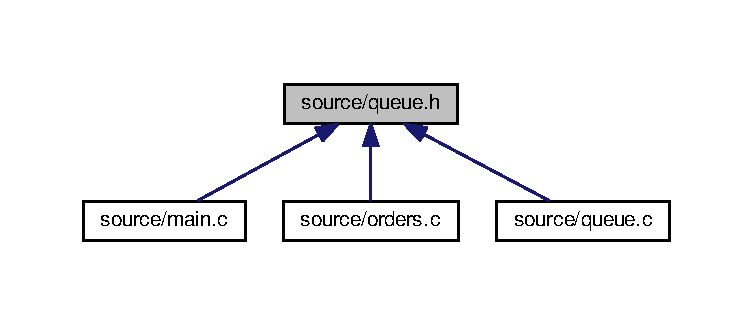
\includegraphics[width=350pt]{queue_8h__dep__incl}
\end{center}
\end{figure}
\subsection*{Typedefs}
\begin{DoxyCompactItemize}
\item 
typedef enum state\+\_\+machine {\bfseries elev\+\_\+state\+\_\+t}\hypertarget{queue_8h_a16ae473719b080c45a88aa7ce3dc9881}{}\label{queue_8h_a16ae473719b080c45a88aa7ce3dc9881}

\end{DoxyCompactItemize}
\subsection*{Enumerations}
\begin{DoxyCompactItemize}
\item 
enum {\bfseries state\+\_\+machine} \{ {\bfseries I\+D\+LE} = 0, 
{\bfseries E\+L\+E\+V\+\_\+\+M\+O\+VE} = 1, 
{\bfseries R\+E\+A\+C\+H\+E\+D\+\_\+\+F\+L\+O\+OR} = 2, 
{\bfseries S\+T\+O\+P\+\_\+\+P\+R\+E\+S\+S\+ED} = 3
 \}\hypertarget{queue_8h_a915b2902e05c4e29541a0e9973500da8}{}\label{queue_8h_a915b2902e05c4e29541a0e9973500da8}

\end{DoxyCompactItemize}
\subsection*{Functions}
\begin{DoxyCompactItemize}
\item 
void \hyperlink{queue_8h_a161ef636c565977af89f20533e0b1f59}{queue\+\_\+remove\+\_\+from\+\_\+queue} ()\hypertarget{queue_8h_a161ef636c565977af89f20533e0b1f59}{}\label{queue_8h_a161ef636c565977af89f20533e0b1f59}

\begin{DoxyCompactList}\small\item\em Removes all orders from current floor from the queue matrix. \end{DoxyCompactList}\item 
bool \hyperlink{queue_8h_ae05a154576e0f550076767a5a9adf9ca}{queue\+\_\+check\+\_\+orders\+\_\+above} (int req\+\_\+floor)
\begin{DoxyCompactList}\small\item\em If the elevator is at a defined floor it checks if there is any orders above, if not it checks if there is any orders above the requested floor. \end{DoxyCompactList}\item 
bool \hyperlink{queue_8h_add57b7ac19f0d6b3e018e9dcb70657da}{queue\+\_\+check\+\_\+orders\+\_\+below} (int req\+\_\+floor)
\begin{DoxyCompactList}\small\item\em If the elevator is at a defined floor it checks if there is any orders below, if not it checks if there is any orders below the requested floor. \end{DoxyCompactList}\item 
bool \hyperlink{queue_8h_a9b768bfd1b03279193f16e9026817ef2}{queue\+\_\+check\+\_\+floor} (int direction)
\begin{DoxyCompactList}\small\item\em Checks the queue matrix to see if the elevator should stop at the floor its passing. \end{DoxyCompactList}\item 
void \hyperlink{queue_8h_a600fb7cf1ff3b028fcb97aa1af196065}{queue\+\_\+reset\+\_\+queue} ()\hypertarget{queue_8h_a600fb7cf1ff3b028fcb97aa1af196065}{}\label{queue_8h_a600fb7cf1ff3b028fcb97aa1af196065}

\begin{DoxyCompactList}\small\item\em Deletes all orders fromthe queue matrix. \end{DoxyCompactList}\item 
bool \hyperlink{queue_8h_a0848377e149d9a178b14d3025a0e1a31}{queue\+\_\+add\+\_\+to\+\_\+queue} (int last\+\_\+floor)
\begin{DoxyCompactList}\small\item\em Updates the programs queue matrix with an incoming order. \end{DoxyCompactList}\end{DoxyCompactItemize}


\subsection{Detailed Description}
Library of functions handling the elevators queue system. 



\subsection{Function Documentation}
\index{queue.\+h@{queue.\+h}!queue\+\_\+add\+\_\+to\+\_\+queue@{queue\+\_\+add\+\_\+to\+\_\+queue}}
\index{queue\+\_\+add\+\_\+to\+\_\+queue@{queue\+\_\+add\+\_\+to\+\_\+queue}!queue.\+h@{queue.\+h}}
\subsubsection[{\texorpdfstring{queue\+\_\+add\+\_\+to\+\_\+queue(int last\+\_\+floor)}{queue_add_to_queue(int last_floor)}}]{\setlength{\rightskip}{0pt plus 5cm}bool queue\+\_\+add\+\_\+to\+\_\+queue (
\begin{DoxyParamCaption}
\item[{int}]{last\+\_\+floor}
\end{DoxyParamCaption}
)}\hypertarget{queue_8h_a0848377e149d9a178b14d3025a0e1a31}{}\label{queue_8h_a0848377e149d9a178b14d3025a0e1a31}


Updates the programs queue matrix with an incoming order. 


\begin{DoxyParams}{Parameters}
{\em last} & floor\+: Last floor elevator visited in order to see if elevator still is in the same floor \\
\hline
\end{DoxyParams}
\begin{DoxyReturn}{Returns}
true if on same floor as last floor and false if not 
\end{DoxyReturn}


Definition at line 24 of file queue.\+c.

\index{queue.\+h@{queue.\+h}!queue\+\_\+check\+\_\+floor@{queue\+\_\+check\+\_\+floor}}
\index{queue\+\_\+check\+\_\+floor@{queue\+\_\+check\+\_\+floor}!queue.\+h@{queue.\+h}}
\subsubsection[{\texorpdfstring{queue\+\_\+check\+\_\+floor(int direction)}{queue_check_floor(int direction)}}]{\setlength{\rightskip}{0pt plus 5cm}bool queue\+\_\+check\+\_\+floor (
\begin{DoxyParamCaption}
\item[{int}]{direction}
\end{DoxyParamCaption}
)}\hypertarget{queue_8h_a9b768bfd1b03279193f16e9026817ef2}{}\label{queue_8h_a9b768bfd1b03279193f16e9026817ef2}


Checks the queue matrix to see if the elevator should stop at the floor its passing. 


\begin{DoxyParams}{Parameters}
{\em direction} & Direction which the elevator is moving. \\
\hline
\end{DoxyParams}
\begin{DoxyReturn}{Returns}
true if there is an order to be handeled on the floor, false if not. 
\end{DoxyReturn}


Definition at line 109 of file queue.\+c.

\index{queue.\+h@{queue.\+h}!queue\+\_\+check\+\_\+orders\+\_\+above@{queue\+\_\+check\+\_\+orders\+\_\+above}}
\index{queue\+\_\+check\+\_\+orders\+\_\+above@{queue\+\_\+check\+\_\+orders\+\_\+above}!queue.\+h@{queue.\+h}}
\subsubsection[{\texorpdfstring{queue\+\_\+check\+\_\+orders\+\_\+above(int req\+\_\+floor)}{queue_check_orders_above(int req_floor)}}]{\setlength{\rightskip}{0pt plus 5cm}bool queue\+\_\+check\+\_\+orders\+\_\+above (
\begin{DoxyParamCaption}
\item[{int}]{req\+\_\+floor}
\end{DoxyParamCaption}
)}\hypertarget{queue_8h_ae05a154576e0f550076767a5a9adf9ca}{}\label{queue_8h_ae05a154576e0f550076767a5a9adf9ca}


If the elevator is at a defined floor it checks if there is any orders above, if not it checks if there is any orders above the requested floor. 


\begin{DoxyParams}{Parameters}
{\em req\+\_\+floor} & Requested floor, only used if the elevator is in an undefined state \\
\hline
\end{DoxyParams}
\begin{DoxyReturn}{Returns}
true if there is an order to be handeled above, false if there are no orders. 
\end{DoxyReturn}


Definition at line 55 of file queue.\+c.

\index{queue.\+h@{queue.\+h}!queue\+\_\+check\+\_\+orders\+\_\+below@{queue\+\_\+check\+\_\+orders\+\_\+below}}
\index{queue\+\_\+check\+\_\+orders\+\_\+below@{queue\+\_\+check\+\_\+orders\+\_\+below}!queue.\+h@{queue.\+h}}
\subsubsection[{\texorpdfstring{queue\+\_\+check\+\_\+orders\+\_\+below(int req\+\_\+floor)}{queue_check_orders_below(int req_floor)}}]{\setlength{\rightskip}{0pt plus 5cm}bool queue\+\_\+check\+\_\+orders\+\_\+below (
\begin{DoxyParamCaption}
\item[{int}]{req\+\_\+floor}
\end{DoxyParamCaption}
)}\hypertarget{queue_8h_add57b7ac19f0d6b3e018e9dcb70657da}{}\label{queue_8h_add57b7ac19f0d6b3e018e9dcb70657da}


If the elevator is at a defined floor it checks if there is any orders below, if not it checks if there is any orders below the requested floor. 


\begin{DoxyParams}{Parameters}
{\em req\+\_\+floor} & Requested floor, only used if the elevator is in an undefined state \\
\hline
\end{DoxyParams}
\begin{DoxyReturn}{Returns}
true if there is an order to be handeled below, false if there are no orders. 
\end{DoxyReturn}


Definition at line 83 of file queue.\+c.


\hypertarget{timer_8h}{}\section{source/timer.h File Reference}
\label{timer_8h}\index{source/timer.\+h@{source/timer.\+h}}


A simple library for doing operations on memory buffers consisting of integers.  


{\ttfamily \#include $<$stdbool.\+h$>$}\\*
{\ttfamily \#include $<$time.\+h$>$}\\*
Include dependency graph for timer.\+h\+:
\nopagebreak
\begin{figure}[H]
\begin{center}
\leavevmode
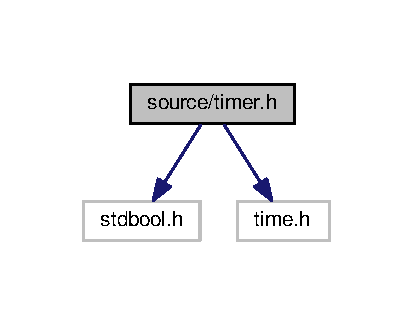
\includegraphics[width=198pt]{timer_8h__incl}
\end{center}
\end{figure}
This graph shows which files directly or indirectly include this file\+:
\nopagebreak
\begin{figure}[H]
\begin{center}
\leavevmode
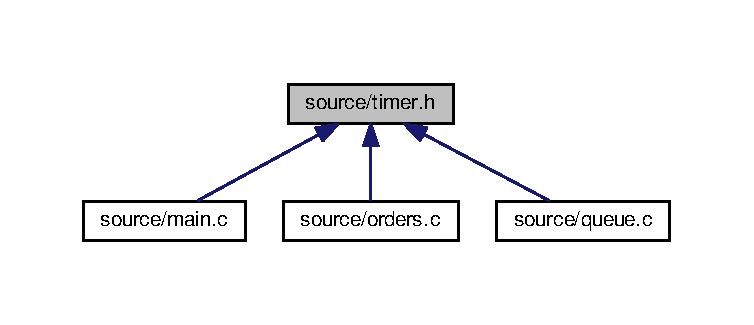
\includegraphics[width=350pt]{timer_8h__dep__incl}
\end{center}
\end{figure}
\subsection*{Functions}
\begin{DoxyCompactItemize}
\item 
void \hyperlink{timer_8h_a232289df78f39fca1fdfc992176a5d75}{timer\+\_\+start\+\_\+timer} ()\hypertarget{timer_8h_a232289df78f39fca1fdfc992176a5d75}{}\label{timer_8h_a232289df78f39fca1fdfc992176a5d75}

\begin{DoxyCompactList}\small\item\em sets m\+\_\+modul\+\_\+timer to current time. \end{DoxyCompactList}\item 
bool \hyperlink{timer_8h_acd10448f170046cdc02ad6af8fb7e7dc}{timer\+\_\+check\+\_\+timer} ()
\begin{DoxyCompactList}\small\item\em Compares the difference between m\+\_\+modul\+\_\+timer and current time to T\+I\+M\+E\+R\+\_\+\+T\+H\+R\+E\+S\+H\+O\+LD. \end{DoxyCompactList}\end{DoxyCompactItemize}


\subsection{Detailed Description}
A simple library for doing operations on memory buffers consisting of integers. 



\subsection{Function Documentation}
\index{timer.\+h@{timer.\+h}!timer\+\_\+check\+\_\+timer@{timer\+\_\+check\+\_\+timer}}
\index{timer\+\_\+check\+\_\+timer@{timer\+\_\+check\+\_\+timer}!timer.\+h@{timer.\+h}}
\subsubsection[{\texorpdfstring{timer\+\_\+check\+\_\+timer()}{timer_check_timer()}}]{\setlength{\rightskip}{0pt plus 5cm}bool timer\+\_\+check\+\_\+timer (
\begin{DoxyParamCaption}
{}
\end{DoxyParamCaption}
)}\hypertarget{timer_8h_acd10448f170046cdc02ad6af8fb7e7dc}{}\label{timer_8h_acd10448f170046cdc02ad6af8fb7e7dc}


Compares the difference between m\+\_\+modul\+\_\+timer and current time to T\+I\+M\+E\+R\+\_\+\+T\+H\+R\+E\+S\+H\+O\+LD. 

\begin{DoxyReturn}{Returns}
True if difference is larger than T\+I\+M\+E\+R\+\_\+\+T\+H\+R\+E\+S\+H\+O\+LD, false if not. 
\end{DoxyReturn}


Definition at line 21 of file timer.\+c.


%--- End generated contents ---

% Index
\backmatter
\newpage
\phantomsection
\clearemptydoublepage
\addcontentsline{toc}{chapter}{Index}
\printindex

\end{document}
